\documentclass[10pt,a4paper,roman, twocolumn]{article}  
%\documentclass[fontsize=10.5pt, twocolumn]{scrartcl}
\usepackage[a-1b]{pdfx}% formato PDF/A, obbligatorio per l'archiviazione delle tesi di Polito
\usepackage{amsmath}
\usepackage{amsfonts}
\usepackage{amssymb}
\usepackage{graphicx}
\usepackage[scale=0.85]{geometry}
\usepackage{color}
\usepackage{hyperref}
\usepackage{enumitem}


\usepackage[font=small,labelfont=bf]{caption}

\setlength{\parindent}{2em}
\setlength{\parskip}{0.2em}


\setlist[enumerate]{topsep=\parskip}
\setlist[itemize]{topsep=\parskip}

\hypersetup{%
	pdfpagemode={UseOutlines},
	bookmarksopen,
	pdfstartview={FitH},
	colorlinks,
	linkcolor={blue},
	citecolor={red},
	urlcolor={blue}
}

\title{\LARGE\textbf{Rethinking Automotive Software Development: Exploring Software Defined Vehicle and its potential}}
\author{
	\textbf{Candidate:} Lorenzo Sciara\\
	\textbf{Supervisors:} prof.~Danilo Bazzanella \\ dott.sa~Piera Limonet
}
\date{}



\begin{document}
\setlength{\belowdisplayskip}{0pt} \setlength{\belowdisplayshortskip}{0pt}
\setlength{\abovedisplayskip}{-0.5\baselineskip} \setlength{\abovedisplayshortskip}{-0.5\baselineskip}

	
\pagenumbering{gobble}
\maketitle
		
\section{Introduction and Motivation}
The \textit{Software Defined Vehicle} (SDV) paradigm is an innovative technology in the automotive industry that, by connecting the vehicle to cloud services and separating software development from supporting hardware systems, allows software to become a fundamental element of vehicle design. The resulting benefits are increased safety and efficiency of automobiles that can be remotely updated over their entire lifecycle using this innovation, and increased efficiency in the production of automotive software, reducing the waste of economic resources and development time.

In the context of the automotive industry, the software produced for vehicles was, until recently, always considered secondary to the production of the vehicles themselves. With the focus on the mechanical parts of the vehicle, software has been very dependent on the hardware for which it was implemented. The software production cycle for a new vehicle consisted of three phases. The development and testing phases were directly performed on the final hardware system. If the system responded correctly, the software was moved to the distribution phase for remaining more or less unchanged for the entire life of the car. Any modifications had to be made physically, resulting in significant resource waste. If the software did not respond correctly, the development and testing process had to be restarted on new hardware, resulting in additional costs and production delays.

The introduction of the SDV completely changes the paradigm. The vehicle's systems are no longer coordinated by special purpose devices related to the system itself, but rather by easily reprogrammable general purpose processors. Additionally, the vehicle is connected directly to the cloud for data analysis and the possibility of receiving \textit{Over The Air} (OTA) updates on any of its systems. At this point, the vehicle becomes a controllable device that can be easily updated based on the data and information it generates, similar to more common devices like smartphones or laptops. This increases both the production efficiency of the software and the safety of the vehicle, since any system vulnerability can be promptly identified, corrected and resolved through updates. Safety is a crucial aspect in the production of vehicle software, so much so that it is considered and classified by the \textit{International Organization for Standardization} (ISO) as a safety-critical device for human life.

In view of these considerations, this thesis aims to provide an overview of the essential elements for creating the SDV and presents a practical project that illustrates its operation with the support of a Raspberry Pi board. The text begins with an overview of the state of the art technologies and approaches currently available, then moves to cloud computing and the advantages offered by \textit{Amazon Web Services} (AWS), and follows with an exploration of the use of AWS services in the context of the project. Finally, this document analyzes the implementation of the project in detail, describing all the development phases and illustrating the support tools used, such as \textit{Hawkbit} for deploying updates to the device and \textit{Grafana} for data analysis.

\section{Contributions of the thesis}

The thesis work's main contributions include defining a \textit{Telematics Control Unit} (TCU) simulator that can emulate the collection of data from vehicle subsystems. Additionally, a basic cloud infrastructure was built using AWS services to receive the telemetry data generated by the simulator and manage the development and deployment of updates on the device. The deployment server was implemented using \textit{Hawkbit}, a tool provided by \textit{Eclipse} that is specifically designed for deploying software to IoT devices. Additionally, a \textit{Grafana} server was implemented for data analysis. The proposed solution integrates elements from the state of the art further advance the field.

To make this solution effective, simplifications were made to the overall SDV concept to reduce complexity. All design and implementation decisions were made while considering the optimal trade-off between available resources and fidelity to the real use case.

The remainder of this section will present the contributions related to the construction phase of the cloud infrastructure -- Cloud Infrastructure -- as the simulator for collecting subsystem telemetry -- TCU Device Simulator -- as the data analysis server -- Grafana Server --. 

\subsection{Service and Allocation Graph}

The first input of the proposed approach is a Service Graph, characterized by a set of network functions such as traffic monitors and load balancers whose behaviour can have an impact on the satisfiability of the Network Security Requirements.

An automatic parser of the input Service Graph has been developed during the thesis, in order to create an internal representation called \textit{Allocation Graph}. Without further specifications, for each link between any pair of network nodes or functions a placeholder -- an \textit{Allocation Place} in the framework -- is generated, so that in this position the optimizer engine can evaluate if a firewall should be placed to reach the optimal allocation schema. 

However, if the service designer has technical knowledge about the security field, he can either force the allocation of a firewall on a specific position without allowing a further removal by the optimizer engine or prohibit the framework to consider a connection between nodes as a potential placeholder for a firewall virtual instance. This capability enriches the potentiality of the proposed methodology, because it offers an extended interactivity with the user and at the same time it decreases the computation time by reducing the solution space the optimizer must investigate to solve the MaxSMT problem, given the addition of some hard clauses. For instance, Figure \ref{fig:stoa} shows how a Service Graph is internally represented in this methodology, supposing that the service designer does not want any firewall between $e_{1}$ and $f_{3}$, while he forces the allocation of a firewall between $f_{4}$ and $e_{5}$.
\begin{figure} [tbh]
	\centerline{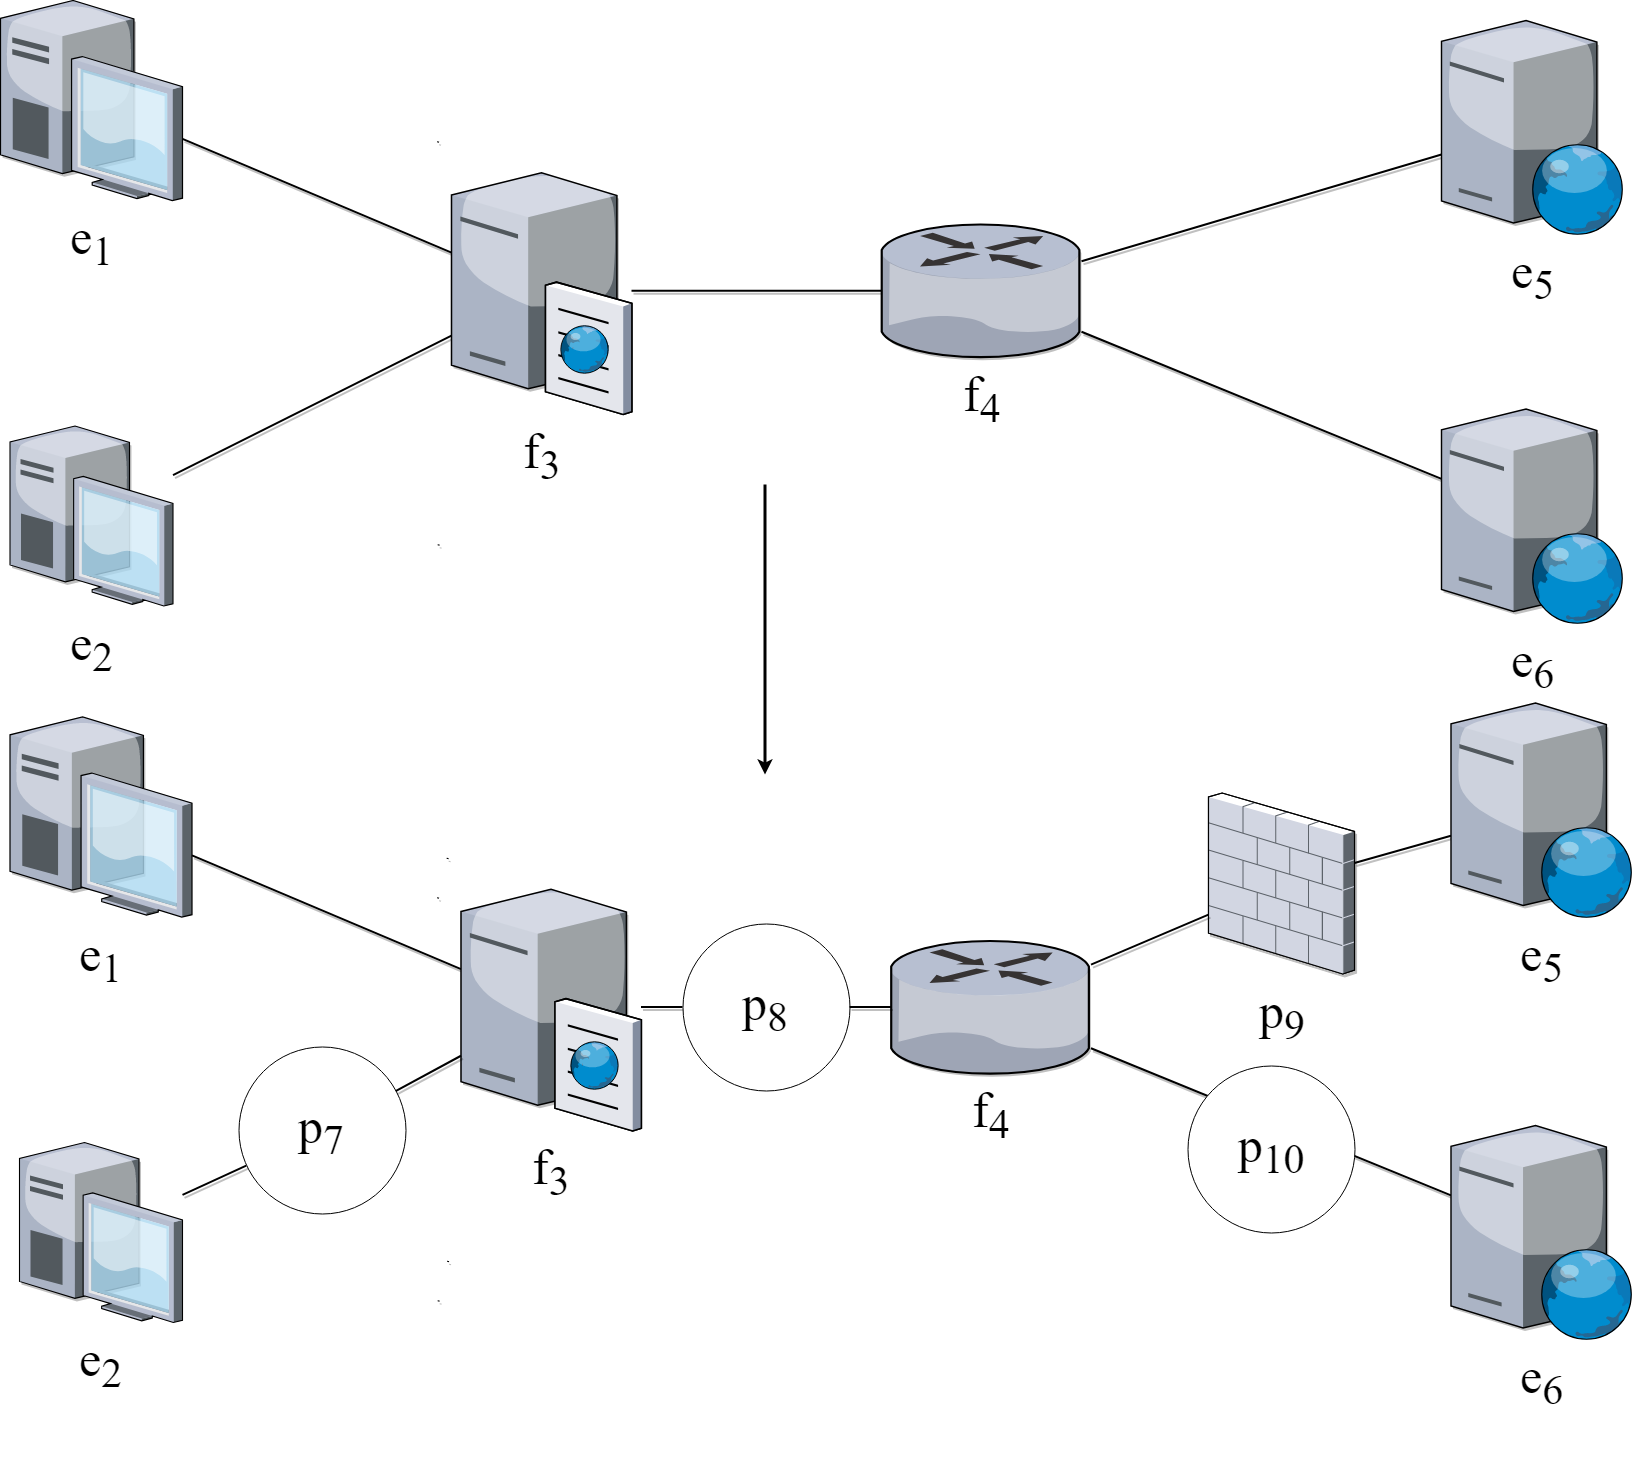
\includegraphics[width=0.4\textwidth]{images/stoa.png}}
	\caption{Automatic generation of an Allocation Graph}
	\label{fig:stoa}
\end{figure}

In this context, a consistent part of the thesis work has been dedicated to the definition of the hard constraints for the forwarding rules of the middle-boxes of the Allocation Graph. The exploited MaxSMT solver -- z3 -- would offer a tool, called \textit{quantifiers}, to express a set of nodes with a single variable and easily create forwarding rules, but it does not put any constraint which would allow to establish the minimum size of this set, with a consequent worsening of the performance the framework could reach. 

The problem which has been challenged, therefore, has been to identify the minimum set of nodes to which a packet can be sent, given a specific port from which it has been previously received, in order to reach the destination. This step has been fundamental to achieve good scalability for the methodology.

\subsection{Network Security Requirements}

The second input is represented by the \textit{Network Security Requirements}, hard constraints which must be enforced in the network to guarantee the required security level. The focus of the thesis was on \textit{connectivity} requirements between a pair of end points. In more details, they can be classified in two different types: 
\begin{enumerate}
\setlength\itemsep{-0.3em}
\item \textit{reachability property}, if a specific traffic flow must be allowed between a pair of end points;
\item \textit{isolation property}, if a specific traffic flow must be denied between a pair of end points.
\end{enumerate}
In this context, each traffic flow is identified by the source and destination IP addresses, the source and destination ports and the transport-level protocol.

In the definitions of the hard constraints representing the NSRs, which are not relaxable clauses because they are necessary conditions to fulfil, some of the aspects which have been considered are the possibility to define bidirectional requirements (e.g. a communication from an end point to another is allowed, while the opposite traffic flow is denied) and to define multiple requirements between the same pair of nodes (e.g. an endpoint can reach another at the destination port 80, while if it tries to contact the port 90 the packets must be blocked). This second example is represented in Figure \ref{fig:multiple03}, where a firewall allows only a specific traffic flow while blocking the others since it is in whitelisting mode.

\begin{figure}[tbh]
	\centerline{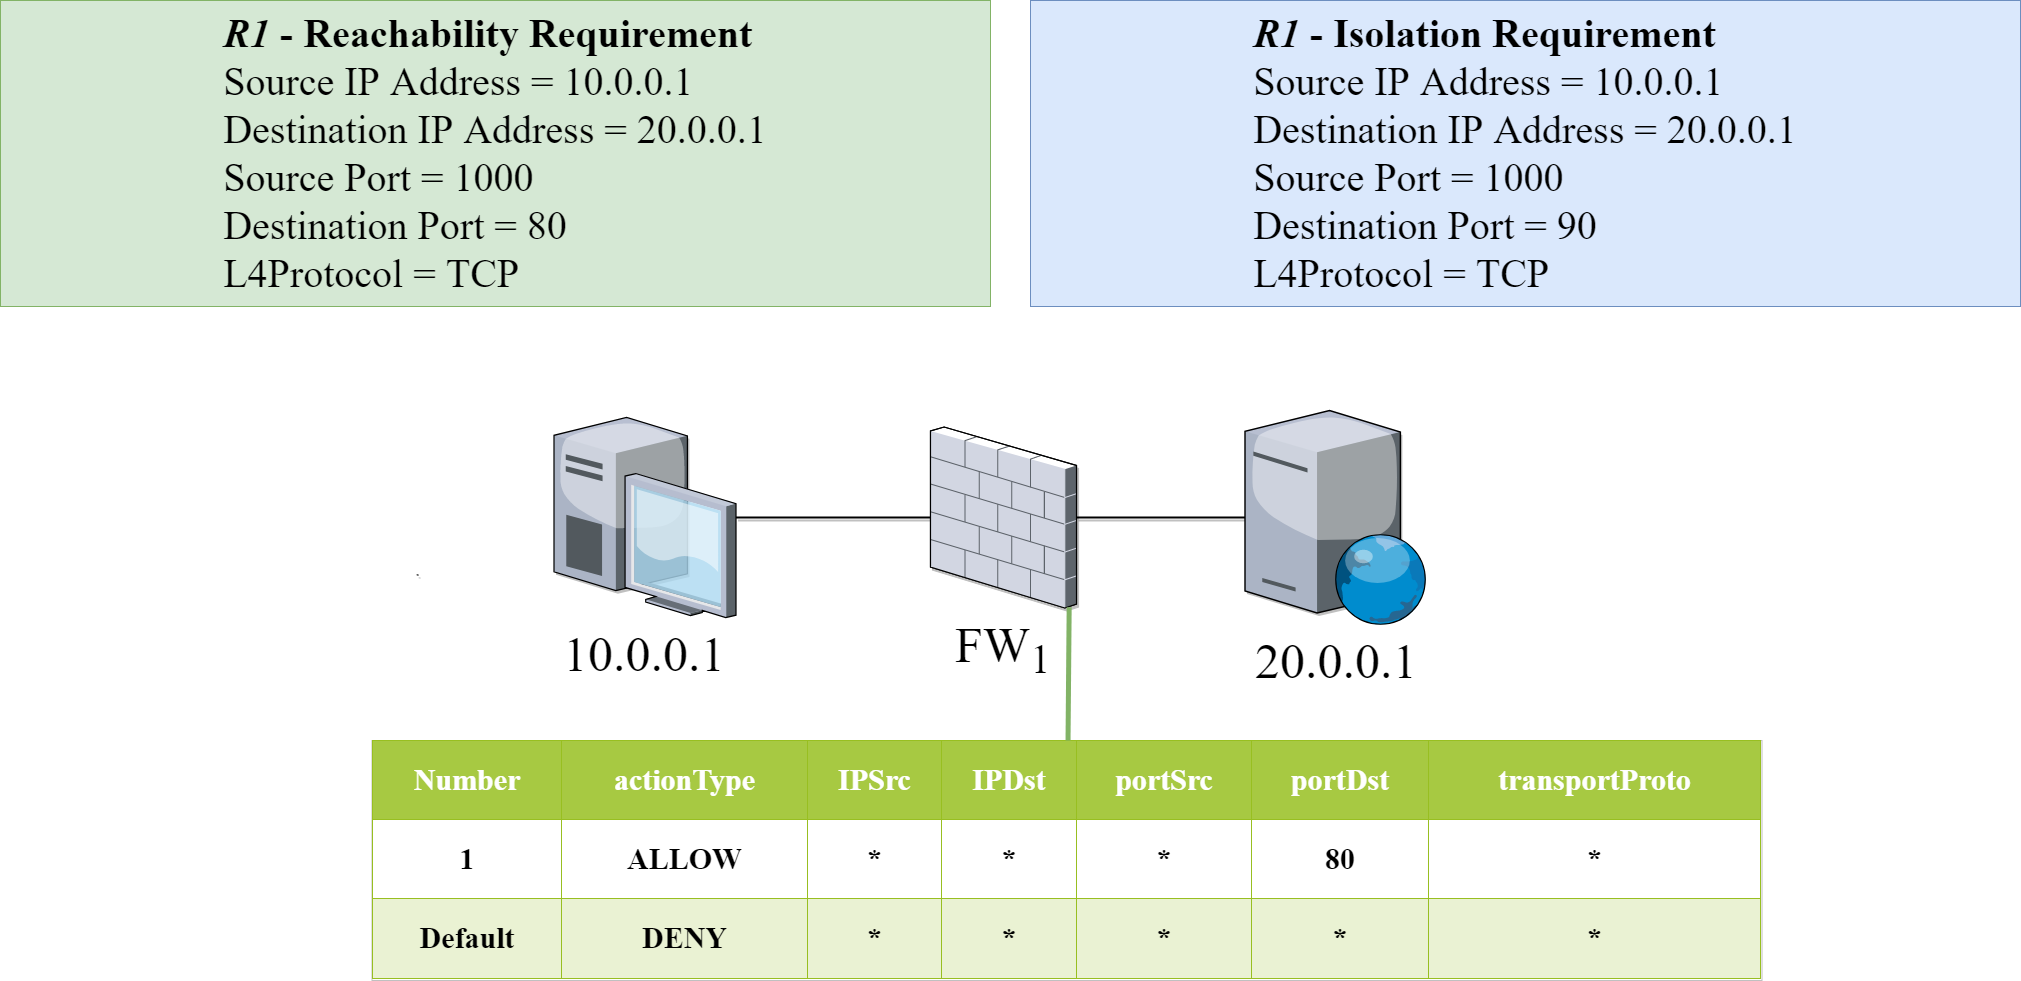
\includegraphics[width=0.5\textwidth]{images/multiple.png}}
	\caption{Example of NSRs between the same end points}
	\label{fig:multiple03}
\end{figure}

\subsection{Packet Filtering Firewalls}

A consistent part of the thesis work focused on defining the soft clauses to reach the optimal allocation of the firewalls in the Allocation Graph and the optimal auto-configuration of their Filtering Policies, that are made by a default action and a set of rules in order to decide if any packet must be forwarded or dropped. The actual objectives which have been modelled are:
\begin{enumerate}
	\setlength\itemsep{-0.3em}
	\item the minimization of the number of allocated firewalls, in order to reduce the resource consumption due to the deployment of the corresponding VNFs;
	\item the minimization of the number of rules for each Filtering Policy, in order to improve the efficiency of the filtering operations. 
\end{enumerate}

About the allocation objective, since the optimal solution would be that there is no need to instantiate VNFs for the packet filtering operation to reduce the resource consumption, then a set of clauses state that it is preferable that in each Allocation Place no firewall is allocated.%, as showed in Formula \ref{fm:soft_place}, where $c_{k}$ is the weight assigned to the corresponding soft clause.

%\begin{equation}  \label{fm:soft_place}
%\forall p_{k}, \; Soft(allocated(p_{k}) = false, \: c_{k1})
%\end{equation}

The critical component of the work has, instead, been related to the auto-configuration of the Filtering Policy rules. Starting from a simple approach where for each NSR the constraints for a corresponding placeholder rule are defined for each allocated firewall, to increase the efficiency of the methodology the thesis contributed to the developing of a number of pruning strategies to reduce the number of placeholder rules: for example, for a specific NSR, a rule is not needed when the default action already satisfies that requirements or when the corresponding traffic flow does not cross the firewall in exam.

A fundamental work has been made on the \textit{wildcards} feature, which allows to represent both an IP address and the netmask in a joint expression: for instance, the $10.0.0.\ast$ statement refers to the network 10.0.0.0/24. The same feature can be applied to transport-level ports and protocols. The idea has been to define the usage of wildcards for each component of the firewall rule as soft constraints, so that a single rule can satisfy contemporary more NSRs by defining larger IP addresses or port  ranges; this way, the solution space can be pruned before the execution of z3 optimizer engine, conspicuously improving the performance. 

Nevertheless, the usage of wildcards for each rule component is less primary than the absence itself of rule inside the firewall Filtering Policy. Consequently, after the definition of all the soft constraints, some time has been spent on the optimal tuning of their weights, so that the optimal solution could be achieved according to the proposed objectives in an efficient way.

\section{Implementation and Validation}

The implementation of the framework has been made by exploiting the Java language, since the z3 theorem prover offers Java APIs to formulate and solve the MaxSMT problem. The interaction with the framework can be made through REST APIs, so that it can be exploited by external tools as a component of a more complex architecture.

This implementation has been, finally, tested extensively in common network scenarios and it showed good scalability against the dimension of the Service Graph and the number of input security requirements. The charts illustrated by Figure \ref{fig:perf01} and Figure \ref{fig:perf02} present the result of a series of tests performed to compare the scalability of the framework implementation related respectively to the number of Allocation Places and Network Security Requirements; in particular, the MaxSAT instances have been solved on a machine with Intel i7-6700 CPU running at 3.40 GHz and
32GB of RAM. 

The first information that can be extracted from the two charts is that the computation time does not increase exponentially either with the number of Allocation Places or with the number of NSRs; this is a very important result, given the computational complexity of the MaxSMT problem. Moreover, the framework scales to Service Graphs of medium-big dimensions, with a high number of links and end points, providing the optimal solution to the presented problem.

It is then possible to notice that an increment of the NSRs number produces a computation time higher than the one produced by the same increment of the Allocation Places number. This result is motivated by the fact that the verification of each requirement must be performed in all the network, considering packets that flow across all the possible paths, whereas the constraints introduced by an additional Allocation Place only impact the traffic flow which crosses that node.

\begin{figure} [tbh]
	\centerline{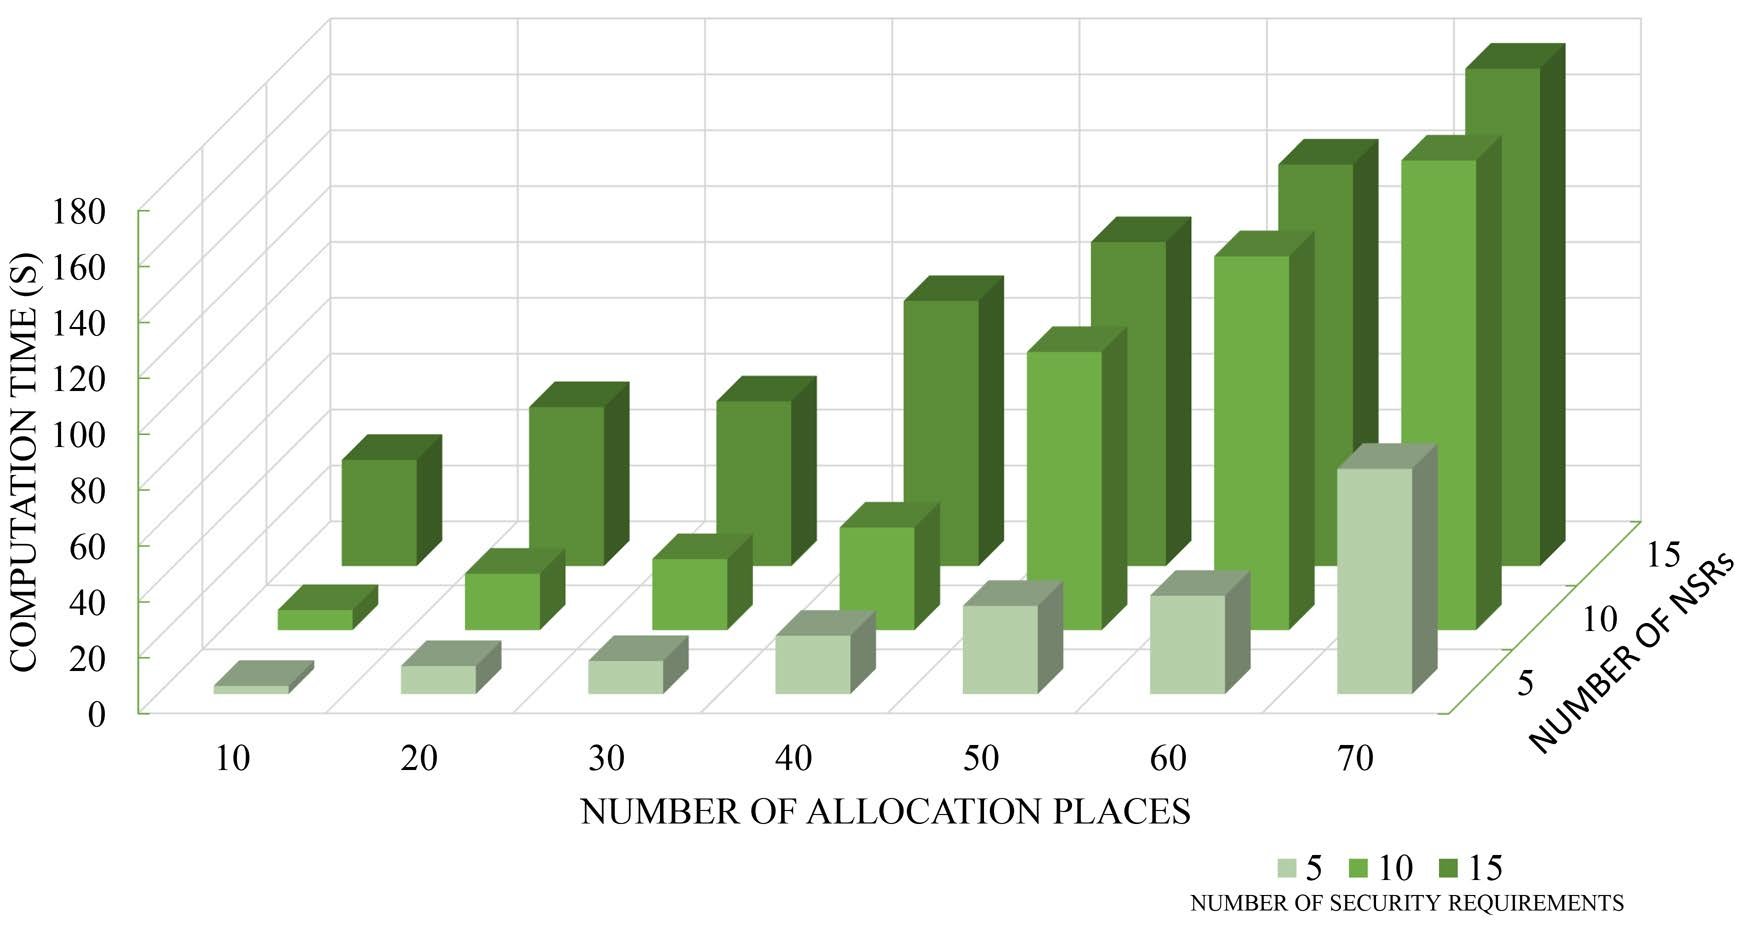
\includegraphics[width=0.5\textwidth]{images/scalability01.pdf}}
	\caption{Scalability tests on Allocation Places}
	\label{fig:perf01}
\end{figure}


\begin{figure} [tbh]
	\centerline{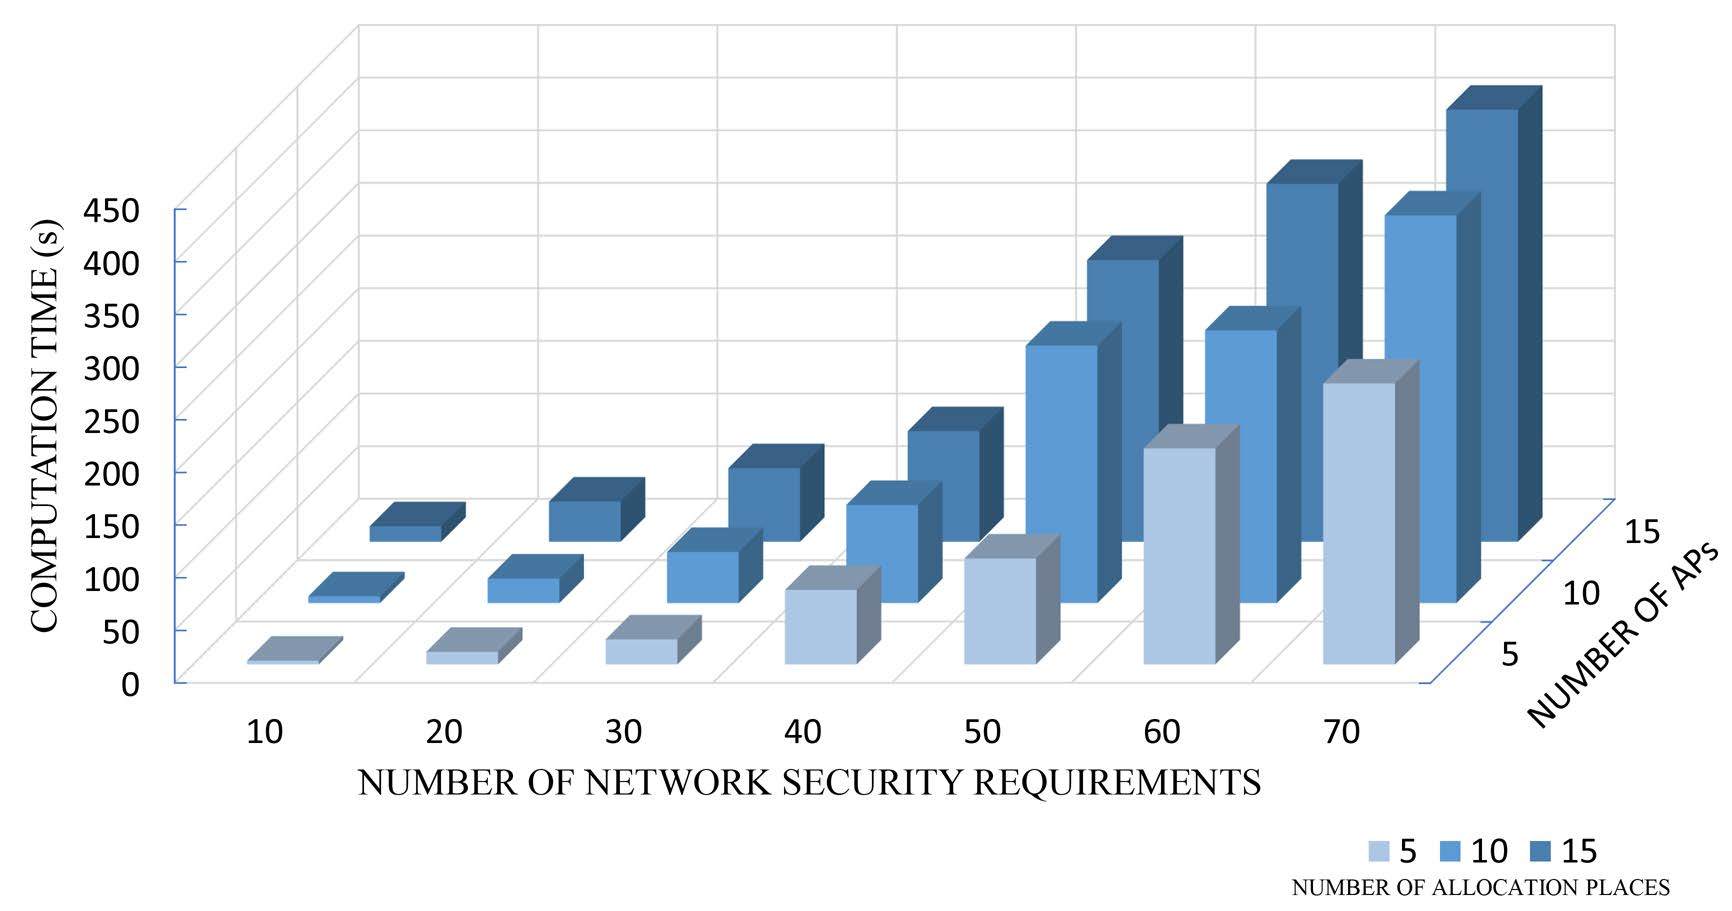
\includegraphics[width=0.5\textwidth]{images/scalability02.pdf}}
	\caption{Scalability tests on NSRs}
	\label{fig:perf02}
\end{figure}

\section{Conclusions and Future Work}
	 
This thesis demonstrates that the proposed approach is feasible and that it can provide a valid alternative in enforcing security functions to manual allocation and configuration of packet filtering firewalls, enabling low latency reaction to changes in security requirements. 

Furthermore, the approach has been developed to be compliant with future extensions such as the support of other NSFs in order to enrich its capabilities. Consequently, in the future the current methodology could be extended to the allocation and auto-configuration of other Network Security Functions, such as anti-spam filter, Web Application Firewall (WAF) and Intrusion Detection System (IDS). %, to further enrich the set of security requirements which can be specified by the user of the framework
Then, another possible future work is represented by the introduction of formal models for other network functions, such as the web cache, which the service designer can exploit to define the Service Graph.

%, on the other side definition of new Network Security Requirement types, which could consider additional features -- e.g. at application layer -- of the traffic flows to allow or to block. The goal would, in fact, be to further enrich the capabilities of the framework.

Finally, this thesis work represented the core content of a conference paper and a journal paper that will be submitted to IEEE/ACM Transactions on Networking in the next months.
	 
\end{document}

